\documentclass[12pt]{article}
\usepackage[utf8]{inputenc}
\usepackage{booktabs}
\usepackage{multirow}
\usepackage{rotating}
\usepackage{bigstrut}
\usepackage{tabularx}
\usepackage{prettyref}
\usepackage{setspace}

%% fonts
\usepackage[utopia]{mathdesign}
\usepackage[scaled=.95]{inconsolata}

%% page margins, inter-paragraph space and no chapters
\usepackage[margin=1.1in]{geometry}
\setlength{\parskip}{0.5em}
\renewcommand{\thesection}{\arabic{section}}

%% bibliography
%\usepackage[american]{babel}
%\usepackage{csquotes}
%\usepackage[style=apa,natbib=true,backend=biber]{biblatex}
%\DeclareLanguageMapping{american}{american-apa}
%\addbibresource{EITC.bib}

%% For actual bib
\usepackage{natbib}
\bibpunct{(}{)}{,}{author-year}{}{,}

%% Fuck with the title
\makeatletter
\renewcommand{\maketitle}{\bgroup\setlength{\parindent}{0pt}
\begin{flushleft}
  \textbf{\@title}

  \@author
\end{flushleft}\egroup
}
\makeatother

%% for memisc
\usepackage{booktabs}
\usepackage{dcolumn}

%% define a dark blue
\usepackage{color}
\definecolor{darkblue}{rgb}{0,0,.5}

%% hyperlinks to references
\usepackage{hyperref}
\hypersetup{colorlinks=true, linkcolor=darkblue, citecolor=darkblue, filecolor=darkblue, urlcolor=darkblue}

\author{Adam Olson\\University of Minnesota\\ \today}
\title{Dissertation Proposal Draft}
\date{February 9, 2014}

\begin{document}
\maketitle

\section{Introduction}
Most scholars who study comparative welfare states refer to the United States as exceptional because they believe any welfare state the United States had was less generous, developed later, and was smaller than welfare states in comparable developed countries (See especially \citealt{andersen1990}). In a very well received challenge to this conventional wisdom, \citet{hacker2002} pointed out, the ``welfare state'' is a contested idea both among political activists and scholars and that not every country provides social policy in a uniform manner. Since then, scholars including Jacob Hacker, Christopher Howard, and others have made a compelling case that what ``is exceptional about the American welfare state is not the level of spending but the source'' of spending \citep[pg. 7]{hacker2002}.

To that point, two prominent forms of social policy in the the United States are visible welfare programs and hidden welfare programs. Visible welfare programs are what most people view as welfare programs in the United States such as Medicare or Social Security. These are programs that are generally well known to politicians, interest groups, and the mass public and they are consistently salient in the national agenda. Traditionally, these are the programs which scholars refer to when they discuss measurements such as welfare effort or welfare spending - they are apparent attempts by the government to alleviate some socially undesirable problem such as poverty or hunger.

Hidden welfare programs, also known as the hidden welfare state, is social policy that is distributes benefits through the tax code as tax expenditures \citep{howard1997}\footnote{A more legalistic definition of tax expenditures is provided in the the Congressional Budget and Impoundment Control Act of 1974 as ``revenue losses attributable to provisions of the Federal tax laws which allow a special exclusion, exemption, or deduction from gross income or which provide a special credit, a preferential rate of tax, or a deferral of tax liability.''}. One prominent example of a hidden welfare program is the Home Mortgage Interest Deduction which was created in 1913 to encourage home ownership which cost the federal government around 100 billion dollars in 2010. This type of welfare through the tax code cost the federal government 1.1 trillion dollars in 2013 which by some estimates is more than was spent on visible welfare programs \citep{omb2013}. Whereas, elderly Americans can apply for social security once they turn 62, then receive a check each month, the hidden welfare state is largely administered through the tax code without much bureaucratic overhead like with Social Security. Like in the visible welfare state, the government tries to alleviate social ills such as poverty or hunger, but it does so in a way that is not evident to most people and generally uses less obvious policy making processes \citep{mettler2011}. 

While our understanding of the hidden welfare state and thus the political aspects of American social policy has increased overall due to the recent work on the hidden welfare state, there remain three sizable gaps in the literature. First, previous literature has studied hidden welfare programs largely in isolation from visible programs. This necessarily produces an incomplete story in trying to understand the politics of American social policy on a broader level. Both visible and hidden programs seek to alleviate some sort of social ill and while specific programs utilize different strategies to accomplish this goal, they remain linked together by this common goal. For example, the United States has several different policies which attempt to provide easier access to housing. Home owners can deduct large parts of their mortgage interest from their federal income tax, the government also provides vouchers to help subsidize rent, and in some cases even provide housing itself. How did America develop a housing policy which incorporates both hidden and visible spending? By examining both hidden and visible programs with similar programmatic goals we can understand how the politics of hidden policies are both similar and different from visible programs in such a way that increases our understanding of American social policy creation and development and the American welfare state overall.

The second gap deals with the idea that policymaking is an iterative process that involves both a creation component \emph{and also} a persistence component. After a policy is created, it has the potential to be expanded or retrenched by enterprising members of Congress (MCs) or bureaucrats. A policy that was created fifty years ago may look nothing like it looks today because of subsequent reforms. This overlaps with the first gap of not considering visible and hidden policies together as a visible policy may be retrenched even while a very similar hidden policy is expanded. Policy affect politics and the tools used to create policy have co-evolved programmatically and politically \citep{schattschneider1960, skocpol1995}.  Historically there has been attention paid to an individual policy's entire life, including after initial passage (see especially \cite{derthick1979, hacker2002}), but most of the theories seeking to explain how the United States developed the welfare state that it did, are only concerned with initial policy creation. 

The third major gap in this type of policy making literature is its inattention to the role of congressional behavior. Research on the American welfare state is strangely devoid of insight from the voluminous literature on congressional policy making. Political Science has tremendous insight as to the role congressional parties, divided government, congressional committees, and many other facets of congressional life have on the behavior of individual MCs and Congress as a whole. While Congress often plays a staring role in scholarly accounts of social policy creation, this research seldom formally incorporates scholarly insight produced by congressional scholars. By applying some of the specific hypotheses outlined by congressional scholars to the historical creation and subsequent development of the American welfare state, we will be able to see how different congressional politics create different policy outcomes. By applying existing congressional literature to the American welfare state literature, we will be able to develop a more dynamic set of predictions for when one type of social policy is created or advanced over another.	

Broadly, this dissertation asks how the United States came to rely on a mix of visible and hidden policies to provide social policy. In pursuing that question, I will draw heavily on the congressional institutions and behavior literature in formulating casual hypotheses. Additionally, it will answer why a legislator utilizes one policy making tool over another to advance their policy goals. Consequently, this dissertation will be able to examine how individual programs are created \emph{and} persist vis-a-vie each other. The juxtaposition of the traditional American welfare state literature, hidden welfare state literature, and also the congressional literature will drastically improve our understanding of how policy is created and changed  based on changing structural and ideological constraints.


%We are beginning to understand how durable traditional policies are under different conditions but do not have a deep understanding of hidden policy durability. (Cite from that patashnik article) 

\section{Literature Review}

The American welfare state literature is rich and well developed, not only in descriptive accounts but also theoretically causal mechanisms as well. Broadly in this section, I discuss both of those parts. In the first subsection, I overview descriptively the American welfare state, focusing on the types of the mechanisms the government uses to provide social policy. In the second subsection, I describe the traditional hypotheses of social policy making in the United States and then discuss several shortcomings of these hypotheses. 

\subsection{What Does American Social Policy Look Like?}
Many scholars have argued that social policy in the United States is exceptional because it lags behind and is less generous than other developed democracies, but it is not the timing or lack of spending that makes America unique, it is the way in which it provides social policy \citep{hacker2002}. Since the end of the second world war, the United States has predominantly used four mechanisms with which to provide social policy: visible spending, regulation, guaranteed rights, and tax expenditures \citep{pierson2007}. All of those mechanisms, but especially tax expenditures have seen explosive growth in the post war period. Tax expenditures are provisions in the tax code that favor or incentive  certain desired behavior and they are functionally equivalent to traditional government outlays or spending. In the United States tax code, there are tax expenditures for everything from buying cars and houses, to having children or working. Once tax expenditures are included in the traditional welfare effort measurement, the United States becomes average in terms of welfare spending when compared to other more `generous' nations \citep[Ch. 1]{howard2008}.

When considering the four described mechanisms of policy provision in the United States, it is important to note that these tools and their resulting policies were not created and are not maintained in isolation from one another. In fact, these tools and policies can work together, exist in conflict with one another, and layer on top of each other. Social policy in the United States seeks to alleviate a social problem. Politicians, based on the political context of the time, will utilize different tools and strategies in an attempt to pass legislation that solves that problem. Of course, political context and perceived political problems are dynamic processes and they change over time -- resulting in a disparate set of policies that seek to solve the same goal, but use functionally different tools.
\begin{figure}[h!]
  \centering
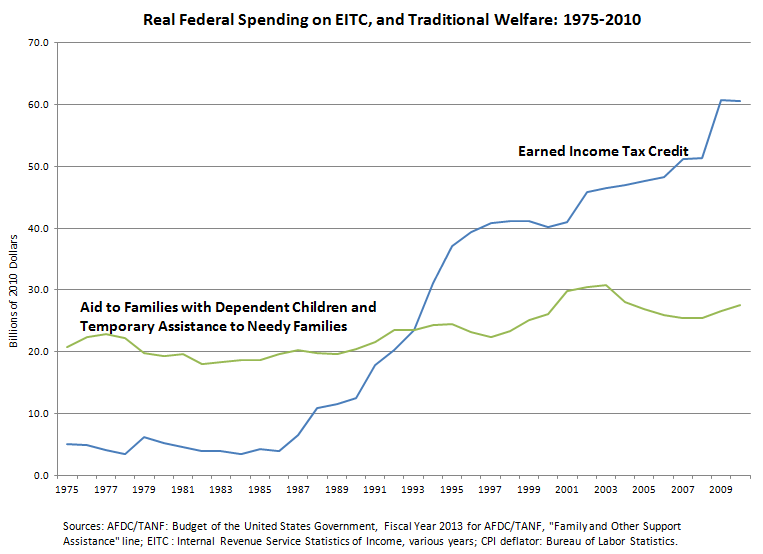
\includegraphics[width=0.9\textwidth]{graph.png}
\end{figure}

Even though tax expenditure spending should be viewed analogously to visible government spending, the politics between the two types of policy are often times quite different and reactive to one another in a way not previously outlined in the literature. One illustrative example is the case of poverty in America. Building on a state run program to provide cash assistance to single mothers, Congress passed Aid to Dependent Children (ADC) which subsidized those state programs for that constituency. By the 1960s, through a series of eligibility changes enacted over the previous thirty years, ADC was the biggest welfare program in the country and served many more types of constituencies than just single mothers. As more Americans became eligible and started receiving ADC, it became increasingly unpopular among the public and elites. Even though the program had never been popular among Americans, it was especially vulnerable to retrenchment in the early years of the Nixon presidency. With the main poverty alleviation program unlikely to be expanded, but with the problem of poverty remaining, elites still wished to legislate around the issue. In 1974 and in spite of the desperately unpopular AFDC\footnote{The program was renamed from Aid to Dependent Children to Aid to Families with Dependent Children during the Great Society period of the 1960s.}, Congress quietly passed a refundable tax credit for the working poor. The Earned Income Tax Credit (EITC) was a wage subsidy for low income people that would zero out their income tax liability and if any of the reward remained, the federal government would send the recipient a check for the remainder. While ADC was never expanded again and ultimately repealed and replaced with a far different program, the Earned Income Credit, social policy through the tax code, was expanded both in eligibility and generosity several times in subsequent decades \citep{stewart1991}. This is clearly seen in the above graph where the EITC explodes in cost relative to AFDC and AFDC remains basically stagnant once the EITC is introduced. The relationship between hidden and visible programs has not been  explicitly discussed in the literature yet we have much to learn from this sort of policy relationship. Why did legislators abandon expansions of ``visible'' welfare spending? Why was there a steady uptick in hidden spending even though it did almost the same thing as the now stagnant visible spending? Ultimately, we do not know why these seemingly similar programs have had such different historical trajectories with AFDC being abolished in 1995 when the EITC, which cost nearly twice as much as AFDC, was left totally untouched and is still used today \citep{myles1997}.

In the 20th century, it is especially within the two spending mechanisms where American social policy worked together and existed in tension with one another to provide services. Over time, these services and policies layer upon one another because political contexts change, which open or close different policy streams, changing the relative effectiveness and impact of the tools used to create policy \citep{kingdon2011}. Sometimes policies are retrenched and removed like in the case of ADC and sometimes the policies surrounding some issue grow and grow because other avenues are closed off like in the case of the EITC. Additionally, that different tools create different types of policies (even though they may serve the same goal), creates different politics. As illustrated above, the politics of visible programs may be radically different from the politics of tax expenditure programs. All of these factors come together to form the spending part of the `exceptional' American welfare state -- a disparate web of interconnected and sometimes competing policies which have layered over time and have been enacted through one of four distinct policy making mechanisms.

With that in mind, this dissertation deals solely with the spending part of the equation, that is visible and hidden spending. The hidden welfare state literature has not been sufficiently linked with the extremely well developed research on the visible welfare state and this dissertation seeks to construct such a link. Additionally, the conventional wisdom as it pertains to the hidden welfare state deals almost entirely with hidden \emph{spending} and analyzing hidden spending vis-a-vie visible spending drastically increases our knowledge of the entire spending component of the American welfare regime. Future research will need to keep broadening the scope of inquiry by including rights and regulation and while they are important in general, they are not important to this story.

\subsection{Why Does American Social Policy Look This Way?}
Having briefly described the mechanisms that the government uses to produce American social policy, we now turn to an overview of why and how the United States created and maintains this type of welfare regime. The United States has a fragmented welfare state with several different types of policies for each goal it tries to alleviate. How did America reach that point? Most research on the American welfare state deals with hypotheses for why the United States has limited \emph{visible} social spending when compared to other developed countries while at the same time, largely overlooking non visible aspects of the welfare system. 

While imperfect, the explanations for the lack of visible social spending in the United States are a good start for discussing policy making overall. These explanations do not account very well what factors lead politicians to utilize one policy making tool over another in either the creation process or the maintenance process. In other words, the conventional theories are static in outlook and are unable to explain why one type of welfare spending increases while another decreases. However, by initially focusing on the conventional wisdom we can clearly draw out these areas that are overlooked.

One school of thought argues that the United States lacks visible spending because American elites and citizens do not want to have a `generous' welfare state \citep{king1973}. The scholars who make this sort of argument generally rely on terms such as political culture or public opinion data to argue that Americans do not believe in a Scandinavian style welfare system. As such, politicians do not feel the pressure to pass that style of welfare and supporting such programs might even be an overall negative for the politician. It is worth noting that support for current welfare programs is relatively high suggesting that American political culture is not a complete explanation for the relative lack of visible welfare spending \citep[Ch. 6]{howard2008}.

Another school of thought argues that the relationship between labor, business and the state is responsible for variation in visible social spending \citep{korpi1980, swenson2004}. This argument, often times called the social democratic model or power resources theory, highlights how the interactions between capital, labor, and the state affected the welfare policy creation process. However, these hypotheses are not in full agreement as to the role of any of these actors. Some scholars emphasize that organized labor had to overcome `naturally hostile' business interests in order to expand welfare programs and that American labor was simply unable to do that. Others argue that large business interests worked with the federal government to create certain welfare programs to offload business expenses to the government. Regardless, these explanations emphasize the role of business and unions (or lack thereof) to explain the creation (or lack thereof) of the American welfare state. 

The third major hypothesis is that the American institutional arrangements create a barrier to passing legislation in general and this drastically reduces the federal government's ability to create expansive welfare policies \citep{pierson1995, robertson2011}. One exceptionally American trait is that the United States has an extremely large number of spots along the policy making process where a proposal's journey can be derailed if a key person or group occupying that location does not support the proposal. The multitude of veto points and those who control such points allows a large number of ways to stop legislation unless veto players are appeased in some way. This includes formal legislative points such as passing a proposal out of committee or overcoming a filibuster as well as less formal elements like interest group support. One prominent way which veto points limited visible spending in the United States is that southern Democrats delayed and reduced welfare spending during the New Deal period in order to ensure African Americans were not able to receive the same level of benefits as whites \citep{katznelson2013}. 

There are several problems with these schools of thought and the literature in general. The biggest problems is that these three schools of thought, as I have said, is that the sole `dependent variable' is visible spending. Obviously one major problem with this oversight is that it does not deal with hidden spending in any meaningful way. Further, social policy creation is occurring in a more incremental way in the United States in the less visible policy arenas. While these canonical theories may be able to explain the New Deal social legislation or the Great Society social legislation they are unable to explain how hidden policies gradually advanced over time. Additionally, they are unable to explain why the legislature adopted a hidden policy over a visible policy (or vice versa) at a given point in time.

Even if the conventional wisdom adopted a more expansive meaning of program visibility, issues of program visibility are not as dichotomous as the emerging research on the hidden welfare state suggests. For instance, program visibility should be considered more continuous than the dichotomous hidden/visible typology suggests. Some policies may be more visible than a tax credit yet less visible than something like social security. Additionally, there are questions of what visibility means to different political actors. When scholars refer to hidden or visible are they speaking about elites or citizens? Lastly, program visibility is not constant and program visibility has the ability to change over time. For instance, President Clinton pushed for large increases in the Earned Income Tax Credit in the early 1990s, suggesting that the program became more visible. Conversely, the food stamp program used to use actual stamps but now uses an EBT card which is basically a debit card, suggesting that the program became more hidden to recipients.

One good way to deal with these problems is to treat social policy as goal oriented rather than focusing on individual policies. For instance, the United States encourages affordable housing in several ways, such as, by allowing home owners to deduct part of their mortgage from their income taxes, providing public housing, providing section eight housing vouchers, and several other policies. By focusing solely on one of these policies (or one type of policy) to the exclusion of the others, we cannot make true inferences about how social policy is made in the United States. It is only through dealing with a collection of policies within a policy goal we will be able to start making generalizable claims about social policy making.

Another separate but related problem is that the conventional theories are largely concerned with policy creation and not subsequent policy development. While policy creation is important, there are two constituent parts of American social policy -- creation and maintenance -- which need to be discussed in attempting to understand the policy making process. The lack of attention to what happens to policy \emph{after} enactment undermines our understanding of the policy making process as a whole especially when policy development can be just as important as policy enactment \citep{patashnik2008}. For instance, if we only concerned ourselves with the creation of Social Security, we would still see a program that excluded large chunks of the population, was largely not a universal program, and still had relatively weak benefits. It was only through post creation development where Social Security became the program we know today \citep{derthick1979}. 


Why would the United States utilize a less obvious form of policy making \emph{instead} of traditional social policy? Why has hidden social policy continued to grow while visible social policy has stagnated? The United States has created lots of hidden policies before, in between, and after, the explosion of visible programs in the 1930s and 1960s yet we do not know why elites chose to use different policy making tools to accomplish their policy goals \citep[Ch. 2]{howard2008}. We also do not know why those hidden programs have been consistently expanded over the 20th century. Additionally, many of the hidden programs created during the non big bang periods had the same goals as the visible programs created in those periods such as encouraging higher education, reducing poverty, or providing health insurance, but we consider individual programs in isolation from the others. It is an important oversight that most conventional research on American social policy does not account for different ways of providing the policy, instead focusing unilaterally on one of the four earlier mentioned mechanisms. If policy is, in a general sense, continually being made, then there is a very large hole in our understanding of American social policy creation because we cannot explain why one type of policy was adopted over another.

\section{The Question of Visible versus Hidden Spending}
With that in mind, this dissertation will argue that the creation and expansion of the hidden welfare state was largely a function of the institutional, ideological, and programmatic visibility constraints on legislative entrepreneurs who wish to advance social policy. The overtime fluctuations in the number of active veto points, institutional centralization, ideological polarization, and program visibility changes the sort of policy tools which have any likelihood of passage. In short, a legislative entrepreneur will choose a social policy making tool which has the best prospect of achieving a winning coalition given the aforementioned constraints of the policy making opportunity.

The logic of this proposition is relatively straight forward. The story of the post war American Congress is one of increasingly strict rules, a more powerful centralized leadership, and more ideological polarization \citep{rohde1991, binder2003}. Additionally, the mid 1970s saw the rise of a new brand of activist conservative who was more aggressive in attacking traditional welfare programs like AFDC and were willing to attack institutional norms to accomplish their goals \citep{hacker2007, theriault2013}. The interaction of more consolidated veto points and more aggressive conservative members of Congress manifested itself in an increasingly hostile environment for traditional social policy. Any potential demand for federal assistance did not dissipate just because of this hostile environment, however, and many legislators still wanted to create and expand more expansive social policies. For some legislators, they found that they were able to quietly get a tax expenditure passed -- often times by attaching it to a much bigger tax bill -- much more easily than they were able to increase traditional welfare programs. Many of the major visible spending programs, which were created during the New Deal and Great Society, became the target of conservative ire which in turn made it more difficult to increase those specific programs. Because of the conservative's ability to leverage institutional constraints to stop such efforts. As these highly visible and unpopular traditional welfare programs stagnanted in legislator driven growth, tax based policies which accomplished very similar goals as the traditional policies began getting popping up and expanding. In turn, as the forces which discouraged traditional policy making (and encouraged hidden policy making) intensified, the same legislators and others wanted to keep advancing their social policy \emph{goals} regardless of policy making \emph{tool}. As such, the tax expenditure route implicit in the hidden welfare state became increasingly the way to advance these goals because it could more easily circumvent hostile veto points.

In this section, I outline some of the forces which specifically influenced the creation and expansion of the hidden welfare state. First, I describe a series of changes in the way congressional rules and behaviors worked over the last fifty years which made passing legislation more difficult and encouraged new ways of policy making. Second, I outline how the rise of a new style of Republican learned to use activist government for their own means. Consequently, changes in institutional rules and individual preferences / tactics intersect intersect to encourage or discourage different policy making tools.

From a broad stand point, ebb and flow of centralized leadership in both houses of Congress is one of the most important factors in encouraging different forms of policy. During the creation of the New Deal and of the Great Society, leadership was in the hands of the committee chairs \citep{shepsle1989}. This allowed rank and file members several different opportunities to peruse their policy goals if they worked within generally agreed upon chamber norms \citep{matthews1960, asher1973}. Strategic politicians could almost `venue shop' between different legislative avenues in their attempt to secure passage of a law. This period of `decentralized leadership' where both chambers relied on reciprocity and committee chairs lasted until the mid 1970s when Democrats started empowering centralized leadership at the expense of committee chairs.

House Democrats in the mid 1970s wished to ``make the people who held positions of power responsible to rank and file Democrats" \citep[pg. 26, quote spoken by Rep. Donald Fraser (D-MN)]{rohde1991}. In pursuing this institutional goal, Democrats passed several intra-party reforms which drastically increased the power of centralized leadership. They stripped many powers from committee chairs and had them run for intra-party election to retain committee chairs. Additionally, many of the powers taken from the committees were placed within central party leadership. The logic behind the internal reforms was to empower the Democratic caucus as a whole and to remove the fiefdoms of deeply entrenched committee chairs. Instead of southern Democrats with lots of seniority setting the agenda, the caucus as a whole got to choose which policies would be advanced in a given Congress. By the 1980s, not only had committee chairs lost most of their powers, the House Democratic caucus began empowering House leadership to negotiate policy on their behalf instead of merely acting as the agent of the party's majority \citep{sinclair1983, palazzolo1992, sinclair1998}.

The transition from a committee based House of Representatives to centralized leadership, empowered by the party as a whole, had profound effects on visible policy making and maintenance. Previously powerful individuals were now unable to exert their previously significant clout to advance their own policy goals. Additionally, members who may have wished to shop a policy idea among several committee chairs lost that ability, having then to appeal to the caucus as a whole. The caucus gained the potential to act an active veto point on individual member policy goals. If policies needed to be supported by the majority of the caucus to have any real possibility of being passed then members with goals in tension with the party faced a real challenge. Moving past the ideological issues, a legislative session has a limited amount of agenda space and time so even if a proposed policy was acceptable to the caucus it still might not be advanced because other things are deemed more important. Before a member who wanted to advance policy goals may have been able to get his idea supported by a powerful committee chair whose power was independent of the caucus. Now, since committee chairs became largely agents \emph{of the} caucus, that proposition became harder.

These House chamber reforms were largely adopted and expanded the Republicans when they won control of both chambers in 1994. With the movement from a committee centric Congress to a speaker centric Congress, conservatives in Congress were able to use the reforms passed by liberal Democrats in the 1970s to their own advantage as well \citep{zelizer2007}. Those with an interest in social policy now faced an even more hostile set of veto points because conservatives controlled the chamber and were actively trying to cut welfare spending whereas previously majority party Democrats may have just not favored expansion. In the New Deal period and prior to the 1970s reforms more generally, the decentralized nature of the House chamber and the lack of well sorted congressional parties encouraged bipartisan and ideologically diverse voting coalitions \citep{poole1997}. This allowed even minority party members to realistically pursue their policy goals. The Republicans who swept into office in 1995 viewed themselves as ideological purists and were largely unwilling to compromise with the now minority Democrats \citep{hacker2006, theriault2013}. Combined with the largely centralized chamber power, Republicans were able to simultaneously pass deep cuts to traditional wellfare programs and also discourage legislators who may have wanted to temper any welfare cuts \citep{aldrich2000}. 

In the Senate, the story is very much the same except it was the reciprocal norm of respect eroding \emph{alongside} the closure of policy making avenues but with a slightly different time line \citep{sinclair1986}. Since the late 1980s, individual senators have spent more resources empowering their party's leadership and those leaders began changing the Senate agenda to maximize inter-party cleavages while minimizing their own party's ideological differences \citep{lee2008}. An obvious consequence of this type of agenda control is that it encouraged ideological sorting among Senators to the point where all conservatives were in one party and all liberals in the other. It was already difficult to pass legislation through the Senate due to supermajority and unanimous consent requirements, so as parties became more homogenized the cost of moving the status quo increased greatly \citep{koger2010}. Like in the House, a costly legislative process encourages members to develop new ways to legislative -- namely, through the tax code.

Outside of individual chambers of Congress, changes in divided government add another potential set of veto points which may could make legislating difficult. Prominently, \cite{mayhew1990} argues that divided government has no real effect on `major' legislation passed in a given Congress. In this case, major legislation means highly salient legislation and by definition does not account for hidden spending. Conversely, divided government has been mentioned as relevant to the creation of hidden welfare spending. \citet[Ch. 4]{howard2008} argues that divided government is associated with more hidden welfare policies being made as it is harder to pass visible legislation in a divided government situation. Since 1970, the United States has had unified government 30\% of the time compared to 70\% for the earlier part of the 20th century. Again, as it becomes harder to pass legislation legislators need to find more innovative ways to advance their policy goals.

While Congress was changing, so to was American conservatism. The rise of the modern American conservative movement came directly as a reaction to the New Deal and the Great Society, and the activist state more generally \citep{critchlow2007, zelizer2010}. In postwar America, the driving conflict between liberals and conservatives was over the scope and size of the federal government within the confines of a New Deal style safety net. Broadly speaking, conservatives wished to retrench New Deal and Great Society programs and generally wanted the federal government to do less but most did not want to remove the safety net altogether. However, the nature and tactics of conservatives started to change in late 1960s though with an increase of conservatives rejecting the ``New Deal Consciousness" \citep{teles2007, skocpol2007}.  

These new style conservatives started getting elected to Congress and just as the 1960s and early 1970s saw a change in tactics among Congressional Democrats, so too did the 1980s see a change in tactics among Congressional Republicans. The Republicans elected to the House of Representatives in 1978 or later showed a distinctly more confrontational style than earlier Republicans. They were willing to utilize any form of House procedure to embarrass or undermine Democratic leaders and were totally unwilling to go along with the ``permanent minority" status that House Republicans had been called during the post-war era \citep{theriault2013}. Whereas Republicans of older generations had reverence for institutional legitimacy, these new style Republicans were willing to destroy institutional legitimacy to gain political power. Slowly and through several successful high profile attacks on Democrats, Rep. Newt Gingrich gained power in the Republican caucus with rank and file Republicans eventually going along with his confrontational approach \citep{harris2006}. 

It was this type of conservative that took over Congress in the 1995 and Speaker Gingrich was able to make the already centralized House institutions even more centralized \citep{roberts2003}. Gingrich changed several House rules to enact preferred policy preferences from the Contract with America. Additionally, the further increase in leadership centralization allowed for ideologically extreme members of Congress to more efficiently use veto points to their advantage. With key leadership positions in the House of Representatives controlled by the `new' brand of conservatives and with the increases in ideological homogeneity, negative agenda control would totally stymie visible policy creation. As with other changes described thus far, lawmakers who wished to advance social policies needed to take a different strategy. This applies to the Senate as well where confrontational Republicans who came up as procedural warriors under Gingrich in the House got elected to the Senate and rapidly started using the looser Senate rules to their advantage to drastically increase both actual polarization and the aggressiveness with which it was invoked \citep{lee2008, theriault2013}.

The evolution and rise of confrontational and ideological conservatism combined with the changes of congressional behavior and rules, I propose, can largely explain the creation and expansion of the hidden welfare state.  Legislatures produce outcomes according to inputs and constraints. As Congress changed so did the types of policy it produced. Overtime, the constraints and inputs changed in such a way which limited certain policy making avenues. Through a rise of restrictive rules, centralized chamber leadership, increased obstruction, increased polarization, and increased ideological extremism, advancing visible spending based social policy through the traditional policy making process became too politically costly for politicians. Legislators who still wanted to advance social policy needed to find other ways to achieve their goals. Consequently, politicians deliberately chose less visible policy making techniques because it was easier for those policies to pass and also become entrenched. By making policy through the tax code, legislators found a tool that did not require as much political capital to advance and was not even on the radar of most other members of Congress. In other words, legislators found a tool that allowed them to circumvent potentially hostile and engaged veto points. 

%talk about visible shit here

The visible component is unique for models of lawmaking and implies that LE policy making tools are differently constrained when some policies are more salient than others at a point in time. Highly salient programs are obviously more well known to constituents and MCs so MCs are more likely to have a well developed opinion on the program or idea. This would encourage opposed MCs to step up their opposition in order to show constituents and other elites that they making good on opposing legislation they disagree with. On the other hand, less visible programs are less salient to constituents and MCs from a . This may allow MCs to have a less developed position on the program or not require them to be as staunch in their opposition as the constituents and other elites may not care. Overcoming passively opposed MCs is much easier than overcoming actively opposed MCs.

It is through the the alternating strength of legislative constraints and changing nature of inputs that the American welfare state was created with related policies layering upon one another, resulting in the `exceptional' fragmented welfare state. The effect of legislators pursuing policies which have a greater chance of getting enacted is that there are several types of policy tools for a given policy goal. More generally, public policy is created over time and is very tightly linked with the institutional arrangements that approve, develop, and administer the program \citep{pierson2004b}. The types of policies that are passed depend on the institutional constraints that the political actors are behaving under and the policy preferences of the actors themselves. By examining the rules and actors involved with a political process -- in this case the creation and development of the American welfare state -- we can illuminate the policy making process, American public policy, and the way political actors and political institutions interact.

\section{Theoretical Expectations}
%A note on coalitions 
\citep{wawro2001}
\citep{evans2004}
The general argument of this dissertation is that ideologically extreme and confrontational members combined with more consolidated legislative veto points causes policy making avenues to become more restricted. Conversely, when potential veto points are more equally distributed among legislators, policy making avenues are more open. To that end, when policy making avenues are more restricted, MCs interested in advancing a policy goal need to utilize policy making tools which circumvent potentially hostile veto players who may hold a disproportionate amount of control of the legislative process. If the veto points are more diffuse, members can more easily attempt to form a coalition by avoiding potentially hostile veto players such as a committee chair.

With that in mind, there are two sets of more specific theoretical expectations that I have in pursuing this dissertation. As the argument relies both on changes in institutions and political actors, it makes sense to outline specific expectations for both components of the argument. In this section, I will outline several expectations concerning the development and creation of both hidden and visible welfare programs as a function of both institutional and individual factors. Consequently, I will delve into when we can expect one type of policy tool to be used more often than a different tool.

\subsection{Institutional Expectations}
The major institutional expectation is that I expect policy creation to vary in conjunction with the conditions outlined by conditional party government (CPG) \citep{rohde1991}. I expect that as the `condition' becomes more engaged -- that is when the two parties are internally ideologically homogeneous and externally polarized from one another -- hidden policy creation will become more common while visible spending creation will lag. \footnote{For the purposes of this dissertation, the condition of CPG is a continuous variable. Over time, the condition becomes more or less met rather than it is either met or it is not met.} Conversely, when the condition is low, that is the parties are ideologically heterogeneous internally and have overlap externally, it will be much easier to pass  and expand visible policy. One of the reasons for this is that more MCs are empowered during periods of low CPG so they are better able to enact their policy preferences. There is no need to hide policy in order to pass it. During high periods of CPG, the reverse is true as fewer MCs are empowered and policy driven members need to think of ways to overcome the consolidated veto points.

In terms of expectations concerning the application of CPG to policy maintenance or growth, I expect efforts at policy expansion to be much more frequent than efforts at policy creation during periods when the condition is more met overall. I expect that policy expansion will be less costly than political creation so MCs focused on policy will focus their efforts on expansion rather than creation. While there may be more attempts at policy expansion, I expect MCs wishing to expand hidden policy to be more effect at enacting their changes than those advocating visible policy expansion. Hidden policies circumvent veto points, whereas visible policies go through a more traditional legislative process. Visible policy expansion is still more subject to stoppage 

Moving away from CPG, I expect that divided government of all types will encourage hidden policy making and expansion, while more unified government will encourage visible policy creation and expansion. While there is disagreement as to the role of divided government in passing legislation, to this argument it is about veto points and tool visibility. In times of divided government, legislators who wish to advance policy goals need to potentially overcome more engaged veto points so they have to resort to hidden policy making tools. During times of unified government, the government is incentivized to pass visible policy so they can claim credit for electoral benefits.

Additionally, I expect coalition durability to be an important factor in visible policy durability but not as important for hidden policy durability. \citet{berry2012} argues that policies are more likely to be retrenched if the party that enacted the policy loses seats in following the enactment. I expect this pattern to apply more to visible policy because a new, potentially hostile regime is more aware of a visible policy. As newer coalitions may be totally ignorant of a hidden policy, I expect those policies to survive coalition changes much more easily. Perhaps expanding them will become more difficult but they are not subject to the same threats of retrenchment as visible policies.

\subsection{Actor Based Expectations}
One assumption of my argument is that hidden policies are pursued because they are less costly politically however that is not true for every member equally. To pursue such a legislative strategy requires the information to know about the policy tool, political power to use such a tool, and ultimately exploit the informational asymmetry. With that in mind, I expect that the actors who are primarily responsible for hidden policy creation to be disproportionately powerful, senior, and electorally safe MCs. The reasoning for this is that I expect to find many hidden programs are created or advanced by last minute amendments or additions to committee reports or floor bills. It would be much easier for people who chair the relevant committee or who have seniority to attach such an amendment without drawing scrutiny from other members. A less experienced member would most likely draw scrutiny with this type of behavior or choose not to do it for other reasons. For instance, it seems less likely that an MC who advocates creating hidden programs would expect significant electoral benefits from claiming credit for the program so I expect MCs who desire reelection as their primary goal to focus on more visible policies. \footnote{
The idea that MCs pursue their goals differently and use policy to achieve reelection is not new \citep{fenno1973, kernell1999}. Regardless, I assume that a legislator that depends on policy advances for election would focus on very high profile legislation.} 

Once a hidden policy is enacted into law, I expect the individual level requirements for expansion of that program to ease all things considered. The rationale is that as a policy remains relatively hidden, any potential political conflict surrounding the policy is largely preempted which ensures that most institutional veto points remain disengaged, requiring less political capital to maintain or expand a program. However, If a hidden program becomes more visible or a visible program becomes even more visible, I expect the individual level political capital costs to increase. If a program is highly visible then members who wish to expand the program must overcome potentially engaged veto points in a way that they would not if the veto players were ignorant of the policy. 

I expect that the ideology of members advancing hidden policy legislation will be more moderate than the caucus average. Fundamentally, I expect the type of legislator who will advance hidden social policy is the type who thinks incremental change is better than nothing and that wide reaching ideological fights are what stop policy innovation. At the same time, I expect ideological extremism to act a multiplier on veto points. As evidences by the increase in more confrontational conservatives, there is ideological polarization but there also the willingness of confrontational members willing to use institutions and rules to their full benefit. I expect that more extremists will drastically cut down on the creation and expansion of visible programs.


\section{Research Design}
The body of the dissertation will be based around the creation and historical development of six individual policies within two separate goal areas of social policy, cash assistance and housing policy. This strategy has numerous benefits. One such being that this strategy allows a research design which combines both within-case and cross-case comparison in a unique two level way \citep{george2005, goertz2012}. As described in Table One, by treating individual policies as cases we are able to examine how institutional and actor changes affected a given policy over time, allowing for within-case analysis. At the same time, we are able to trace individual policy creation development in relation to other policies in the same policy area, allowing for cross-case comparisons. Similarly, when we treat policy area as the unit of analysis, we can examine how a policy area changes over time and how policy areas developed in relation to one another. By using this type of case study approach, I am able to develop a very flexible broad based approach to this dissertation where we can see how policies and policy areas developed and changed in response and alongside one another. 

%lol this table looks super bad in code. Don't ever change it.

\begin{table}
\centering
    \begin{tabularx}{\textwidth}{XXX} \toprule
           & \textbf{Within Case Comparison} & \textbf{Cross Case Comparison                                                                              } \\ \midrule
    \textbf{Individual Policy Level} & Trace Creation and Development of Individual Policies        & Compare Creation and Development of Individual Policies against other policies within a policy area \\
    \textbf{Policy Area Level}       & Trace Creation and Development of Policies in a Policy Area as a Whole & Compare Creation and Development of Policy Areas against other Policy Areas                         \\ \bottomrule
    \end{tabularx}
  \caption{Multi-Level Case Study Design}
  \label{tab:casestudy}
\end{table}

Those six policies used for this dissertation, described in table two, are representative of the type of spending policies that politicians choose to utilize in providing social policy. In selecting policies to analyze, one must be careful to ensure the method of policy making represents a wide swath of options available to policy makers. Considering this, I have chosen policies within a goal area to represent the array of individual policies a politician may choose to advance their policy goal. Since legislators care about policy goals, they will choose whatever tool allows them to advance that goal. The three policies per goal represent those options. 

Additionally, the goal areas and individual policies are often times what people mean when they say welfare which allows for external validity. Much of the previous literature on welfare state creation and maintenance deals with health care policy or pension policy, but there is less on dealing with this cash assistance or housing policy from a policy development. To be sure, they are well studied policies but we only understand them on an individual level basis. As such, do not know why, for instance, we would see an expansion in one type of cash assistance (EITC) but not another (AFDC). These goal areas lead themselves to this type of analysis very well.

\begin{table}
\centering
    \begin{tabularx}{\textwidth}{XXX} \toprule
           & \textbf{Housing Policy} & \textbf{Cash Assistance Policy} \\ \midrule
    \textbf{Traditional Social Policy} & Public Housing        & Aid to Families with Dependent Children \\
        \textbf{Mixed Social Policy} & Housing Choice Voucher Program        & Supplemental Nutrition Assistance Program \\
    \textbf{Tax Based Social Policy} & Home Mortgage Interest Tax Deduction        & Earned Income Tax Credit \\ \bottomrule
    \end{tabularx}
  \caption{Types of Policies According to Policy Tool Area}
  \label{tab:types}
\end{table}

From a broad stand point, this dissertation will examine both macro trends in social policy making and maintenance along with trends in individual policies within two distinct social policy goal areas. In pursuing that strategy, this dissertation will use a combination of quantitative and qualitative methods in order to make it's case that certain changes in institutions and behaviors encourage one type of social policy making over another. Additionally, this dissertation will extend over a wide swath of the 20th and 21st century enabling the ability to examine changes in social policy making against the backdrop of changes in the congressional behavior and institutions.

More specifically, this dissertation will use both quantitative and qualitative methods and data, presenting itself in a mixed methodology dissertation. At every step of the way, I hope to combine both a qualitative and historical narrative punctuated with sophisticated statistical analysis. Quantified measurements of interest such as program visibility will be utilized throughout. The dissertation will begin with a quantitative examination of visible versus hidden social policy trends over the last several decades, showing that visible policies have stagnated (or declined) while hidden policies have exploded. This presents the empirical puzzle, sets the stage for subsequent analysis, and also continues to fill the gap in American social policy literature by showing that substantial parts of the American welfare system are distributed through the tax code. Additionally, it helps show that the growth of more visible polices are in a dynamic relationship with hidden policies where policies might change in reaction or in tandem to one another. By pairing the larger spending analysis with two large scope case studies, we create a methodological strategy where we examine the same policies and politics through different lenses, bringing even more insight.

As with the overview section, analysis of the case studies and policy goals will use both quantitative data alongside qualitative data. The role of constructing a narrative is important in the case studies because it will allow us to highlight relationships not easily uncovered with traditional data analysis. When dealing with such large stretches of history -- in one case back to at least 1913 -- with many different moving parts, it makes sense to tell the theoretical story qualitatively and provide quantitative evidence at key points in the story. I envision using the following types of data to help provide this evidence:
\begin{itemize}
\setlength{\itemsep}{-2pt}
\item Roll call vote data
\item Cosponsor data
\item Bill characteristics data including sponsor characteristics, how far the bill advanced, number of cosponsors.
\item Committee vote data
\item Speech data including non legislative speech, debate speech, committee speech
\item Roll Rates
\end{itemize}
These data are the quantified outcomes of what happens in Congress on a day to day basis. Broadly, these data allow us to measure both individual level behaviors in a party controlled environment. We are looking for both how the party constrains the actor and how the actor overcomes (or does not) those constraints. For instance, do we see that a very senior member is rarely on the losing side of a floor vote yet maintains a moderate ideology? That member might be a strong candidate for someone who advances hidden legislation. Do we see a member who routinely gives bombastic speeches on the House Floor, is often on the losing side of a vote, and does not get many cosponsors for their proposals? That member might be the sort of member that exacerbates polarization and engages veto points.

Additionally, many of the hypotheses require proxies for relevant quantitative analysis. The way we generally measure ideology in Congress is with NOMINATE scores \citep{poole1997}. A significant swath of this dissertation deals with ideology such as CPG, extremism, and moderation. This will be the measurement for ideology that I use. When CPG was first developed, \cite{rohde1991} used Americans for a Democratic Society voting scores to create his party homogenization and heterogeneous measurements. I will use NOMINATE as a replacement.

Moreover, another major part the dissertation deals with potential veto points. Of course, having to choose which veto points matter is an important consideration. In choosing which veto points matter, I rely on three sources: \cite{krehbiel1998}, \cite{schickler2001}, and \cite{koger2010}. \footnote{I'll add these to the next draft in appendix form.} \cite{krehbiel1998} lays out the idea of pivotal members, that is, the member who essentially decides if a bill is advanced or not. There are pivots at every step of the legislative process -- committee, floor, filibuster, etc. More specifically, \cite{schickler2001} and \cite{koger2010} outline explicit institutional changes which result in veto point changes or types of obstruction that a proposal must overcome. Obviously not every possible veto point will be relevant at all times, but it seems better to start with a broader list and identify potential bottlenecks ahead of time to see how legislators avoid them. Implicit to the discussion of veto points and polarization in my argument is the consolidation of veto points as a consequence of leadership centralization. One part of my argument is that when veto points are consolidated in actors, the tools that other actors use to advance their policy goals change. By using the previously discussed sources, but especially \cite{schickler2001}'s expansive list of institutional changes, I can chart how veto points are distributed among legislators over time.

It is also useful to examine how I will construct original measurements when necessary. One specific case of this is that I outline program visibility in a way not before done which allows for visibility to be different between elites and regular people. My version of visibility also has the ability to change over time which means a regular measurement is required. For measuring program visibility to elites, congressional speech or bill introduction / co-sponsorship would serve as a good measurement of salience. It is relatively straight forward to collect data about bills that deal with hidden policies and searching technology in speech makes collecting congressional speech straight forward as well. Program visibility to regular people would measured by newspaper editorials.

Pivoting, one benefit to this sort of research design and argument is that most of the argument is generalizable to different temporal eras with some caveats. One such caveat is that there is a basic level of temporal comparability and traceability between the eras used in analysis and any proposed era of analysis. For instance, while there is evidence that there was federal social policy such as regulation and welfare prior to the New Deal, the relationship between these tools was likely very different then compared to now, as the country existed in a different party system, hadn't yet engaged in either world wars, in addition to many other differences \citep{skocpol1995, balogh2009}. That is not to say that pre-New Deal is unusable -- indeed, I will go back that far because the Home Mortgage Interest Deduction goes back that far -- but a steady hand will be required when examining contextual, institutional, and behavioral factors.

Another such caveat in judging generalizability is that the contrast between \emph{traditional} and \emph{`hidden'} policy is not necessarily the important quantities of interest. What is important is the contrast between politically expensive and inexpensive policy making tools. For instance, it is entirely plausible that legislators will eventually overuse the tax policy route of creating and expanding social policy when it becomes too salient to the public and legislators. Politicians use less salient or hidden means to create policy because fewer veto players are cognizant of that form of policy making. As I mentioned at the start, \cite{pierson2007} outlined four types of policy tools used by legislators. This dissertation argues that the major two tools of the 20th century are tax policy and traditional spending. Pierson also notes, however, that there are steady increases in guaranteeing rights as well as regulation. With that in mind, if passing `hidden' legislation becomes as difficult as passing traditional legislation, I fully anticipate innovative legislators will pursue different strategies such as trying to advance technically complicated regulatory bills or pressuring bureaucrats to do things instead of focusing on statutory innovation. \footnote{I think this point might be happening sooner than we think. It seems as though legislative output of all forms is significantly decreased since the rise of the Tea Party and with President Obama vowing to advance his causes unilaterally, it may be time for legislators to think of some new way to advance legislation} 

One drawback to this style of research design is that it relies on a collection of data sources, narratives, and interpretation to develop the argument. While in many ways it may be a strength to build a case upon a collection of sources, such a strategy lacks scientific rigor in the traditional sense \citep{king1994}. Regardless of these claims, it is more difficult to find causal links with this sort of research design than it might be with a less ambitious set of arguments, thus raising the bar for me. Hopefully this increased difficulty produces a better document overall which persuades more people because of the methodological pluralism contained within.

Regardless of the relative merits of the research design, I envision it being relatively similar to both \cite{zelizer1998} and \cite{schickler2001} in tandem. \cite{zelizer1998} examines the structural constraints on long time House of Representatives Ways and Means Chairman Wilbur Mills and how they shaped the types of policies he pursued (and also his attempts at changing the constraints). Zelizer is an academic historian so his book is largely concerned with constructing a narrative about Mills and these constraints through time. I am looking at the question of choosing which legislative tool through the same sort of lens. Some constraints encourage different behavior and politicians react accordingly. Additionally, \cite{schickler2001} tells a story about how diffuse interests come together at different points in Congressional history to change the institutional rules and constraints. His work is largely historical in outlook as well, but he shows the effect of some of those interests using traditional quantitative analyses such as regression. I anticipate that sort of strategy will be extremely helpful towards my dissertation.

Overall, the research design for this project is flexible enough to account for many covarying parts while remaining powerful enough to tell a causal story. By combining a multitude of primary, secondary, quantitative and qualitative data sources I will be able to weave a strong multi-methodology dissertation which does not rely too heavily on one particular analysis to make an argument. Additionally, by using several different units of analysis, this dissertation will be strongly positioned to isolate relevant causal factors in the pursuit of identifying reasons why MCs choose to advance one form of policy over another. An additional benefit to that form of research design is that it strongly positions the dissertation to tell a readable and compelling narrative to underlay the analyses in the document. 

\section{Chapter Outline}
\begin{description}
\item[Chapter One] The first chapter would introduce the puzzle and overview the theory. In the first part of the chapter, I will present the idea that hidden policies have continued to grow while visible policies have stagnated. In the second half of the chapter, I will show variability in policy visibility. Both these parts set the stage nicely for the theory that politicians seek the path of least resistance when pursuing a goal oriented social policy strategy.
\item[Chapter Two]
\item[Chapter Three]
\item[Chapter Four]
\item[Chapter Five]
\end{description}

\newpage
    \bibliography{EITC}{}
\bibliographystyle{jpe}

%\printbibliography
\end{document}

